\documentclass{article}
\usepackage[a4paper, hmargin={2.8cm, 2.8cm}, vmargin={2.5cm, 2.5cm}]{geometry}
\usepackage{graphicx}
\usepackage{caption}
\usepackage{amsmath}
\newtheorem{myex}{Example}
\newtheorem{mydef}{Definition}
\begin{document}
\subsection{Nucleic Acids}
((TODO: TELL WHY NUCLIEC ACIDS))
\subsubsection{Ribonucleic acid} %NEEDS FIGURES
((TODO: ADD FIGURES, TALK ABOUT DIFFERENT KINDS OF RNA))\\\\
%RNA is massproduced
Ribonucleic acid (RNA) is a large molecule composed of nitrogenous 
bases nested on a ribose-phosphate backbone. The possible nitrogenous bases, or 
bases for short, 
that can be nested on the backbone are guanine (G), adenine (A), uracil (U) and cytosine 
(C). In nature, the predominant form of RNA are as a singlestranded chain 
that can fold in on itself, bundled with other chains to form a structure. 
This flexibility of the backbone that allows for the chain to fold in on itself 
is possible because the RNA uses a sugar called ribose in its backbone, 
which is unstable compared to its other form, deoxyribose, used in 
deoxyribonucleic acid (DNA), but is more flexible, allowing the RNA chain to 
bend in ways that DNA can not.\\

The bases found in RNA can form hydrogen bonds with each other, though not all 
bases can form bonds with each other. Bases that can bond with each other are 
guanine with cytosine, and adenine with uracil. These bonds are complementary 
of each other, and forms the structure of each RNA. When 
two bases bond with each other, they will stick to each other 
which changes the form of the RNA chain. However sometimes a base will have no 
complementary base to bond with, causing the base to stick out, giving rise to 
certain characteristic forms. This will be elaborated on later.
%Source: http://en.wikipedia.org/wiki/RNA accessed 18/05-2015 12:10

\subsubsection{Deoxyribonucleic acid}
((TODO: ADD FIGURES, TELL MORE ABOUT DNA))\\\\
%DNA is produced for sharing and is maintained
Deoxyribonucleic acid (DNA) is a large molecule composed of nitrogenous bases 
nested on a deoxyribose-phosphate. DNA is mostly found in nature as helixes, 
where two strands has bonded. Similarly to RNA, DNA has four nitrogenous 
bases, and shares three of the four that RNA have, (guanine, adenine and cytosine). 
However instead of uracil, the fourth base is thymine (T). 

%Source: http://en.wikipedia.org/wiki/DNA accessed 18/05-2015 12:28


\subsubsection{Secondary Structures of Nucleic Acids}
The secondary structure of a nucleic acid describes how the bases of the 
nucleic acid has bonded. The secondary structure of nucleic acids can change if 
the nucleic acid is damaged or has mutated, causing it to gain or lose 
bases. When two bases bonds they hold onto each other, causing bases that 
have no complementary base to bond with to stick out. Below are examples of three 
common secondary structures as well as a brief analysis on how to identify them.\\\\
\textbf{Bulge}\\ 
A bulge occurs when one or more bases have no base to bond with and these 
bases are surrounded by bases that have bonded. This causes the bases to get 
pushed out slightly, resembling a bulging growth. This type of structure occurs 
when one or more bases has been inserted or deleted, since if a base has been 
inserted then it will have no base to bond with, and if a base has been deleted 
then the previously-bonded base will have no base to bond with. 
Below is an example of a bulge:
\begin{myex}\centering
\begin{figure}[h]
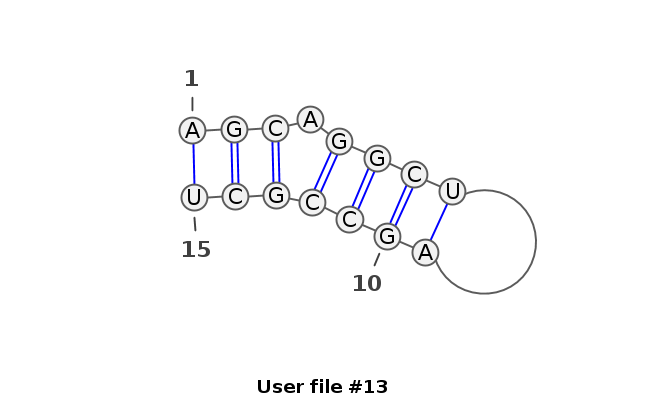
\includegraphics[scale=0.4]{bulge.png}
\end{figure}
The RNA sequence {\tt AGCAGGCUAGCCGCU}. Note the bulging {\tt A}.
\end{myex}
Since we know that a bulge occurs when a base is inserted or deleted, we can 
define a bulge as follows:
\begin{mydef}\centering
Let S be a bulge. Let $E$ be a sequence of characters. Let $\Sigma$ be an alphabet. 
Let $a \in \Sigma$. Let $0$ be the empty string. Let $\Lambda$ be a map that holds the complement to each 
base described in the alphabet. Let $E^{-1}$ denote the reverse of the sequence. 
Then we can define a stem loop as follows;
\begin{align*}
S    &= E'~f(E^{-1})~|~E~f(E^{-1\prime})\\
E    &= \{a\}~E~|~0\\
E'   &= E~E'~|~E\\
f(E) &= \Lambda(E)
\end{align*}
\end{mydef}
((NOTE: ABOVE DEFINITION NEEDS WORK, ISN'T CORRECT))\\
\\\\
\textbf{Interior Loop}\\
An interior loop is when two or more opposing bases aren't complementary and 
can't bond, causing them both to bulge. This occurs when one or more 
consecutive bases mutate to another base, or there has occured a deletion or 
insertion on both sides of the strand on the same spot. Below is an example of an interior 
loop:
\begin{myex}\centering
\begin{figure}[h]
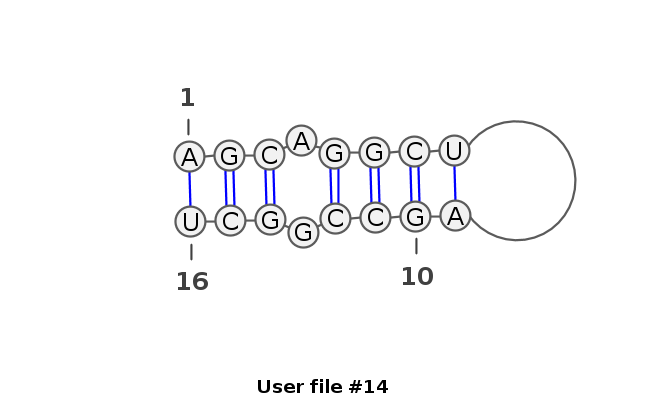
\includegraphics[scale=0.5]{interior-loop.png}
\end{figure}
The RNA sequence {\tt AGCAGGCUAGCCGGCU}. Note the bulging {\tt A} and {\tt G} 
creating a loop inside the bonded strand.
\end{myex}
These interior loops vary in size, and can have differing amount of bases on 
either side of the strands, making them hard to generalize.\\
((TODO: ADD A BETTER EXPLANATION AND A DEFINITION OF AN INTERIOR LOOP))
\\\\
\textbf{Stem Loop}\\
A stem loop, also known as a hairpin loop, occurs when a strand bonds with 
itself, but leaves a sequence of bases sticking out that doesn't bond with anything. 
This kind of loop occurs typically in RNA as they are single-stranded, but may 
happen in DNA if the two strands of the DNA has been separated. Below is an 
example of a stem loop:\newpage
\begin{myex}\centering
\begin{figure}[h]
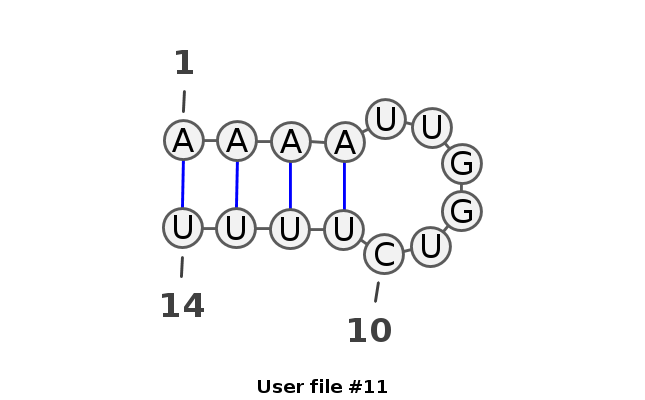
\includegraphics[scale=0.5]{stem-loop.png}
\end{figure}
A stem loop of the RNA sequence {\tt AAAAUUGGUCUUUU}.
\end{myex}
An important thing to take note of is how the sequence can be seen as one 
long strand that starts from the adenine bases that binds with the uracil bases, 
loops around without binding to anything and finally become the uracil bases 
that the adenine bases from the start binds with. This means that the 
stem loop can be written as one continuous sequence of bases; {\tt AAAAUUGGUCUUUU}. 
This specific kind of loop adheres to a specific pattern that reflects from 
the example, that can be defined as follows:
\begin{mydef}
\centering
Let S be a stem loop. Let $E_n$ be a sequence of characters. Let $\Sigma$ be an alphabet. Let 
$a \in \Sigma$. Let $\Lambda$ be a map that holds the complement to each base 
described in the alphabet. Let $E_n^{-1}$
denote the reverse of the sequence. Then we can define a stem loop as follows;
\begin{align*}
S      &= E_0 E_1 f(E_0^{-1}) \\
E_n    &= \{a\}\\
f(E_n) &= \Lambda(E_n)
\end{align*}
\end{mydef}
Since we can define a stem loop we can, with the right tools, search through 
a file documenting the bases of a nucleic acid and find all stem loops 
the nucleic acid has.
\end{document}

